%-----------------------------------LICENSE------------------------------------%
%   This file is part of tikz_figures.                                         %
%                                                                              %
%   tikz_figures is free software: you can redistribute it and/or              %
%   modify it it under the terms of the GNU General Public License as          %
%   published by the Free Software Foundation, either version 3 of the         %
%   License, or (at your option) any later version.                            %
%                                                                              %
%   tikz_figures is distributed in the hope that it will be useful,            %
%   but WITHOUT ANY WARRANTY; without even the implied warranty of             %
%   MERCHANTABILITY or FITNESS FOR A PARTICULAR PURPOSE.  See the              %
%   GNU General Public License for more details.                               %
%                                                                              %
%   You should have received a copy of the GNU General Public License along    %
%   with tikz_figures.  If not, see <https://www.gnu.org/licenses/>.           %
%------------------------------------------------------------------------------%

% Use the standalone class for displaying the tikz image on a small PDF.
\documentclass[crop, tikz]{standalone}

% Import the tikz package to use for the drawing.
\usepackage{tikz}

% Tikz packages used.
\usetikzlibrary{decorations.markings, arrows.meta}

% Begin the document.
\begin{document}

    % Draw the figure.
    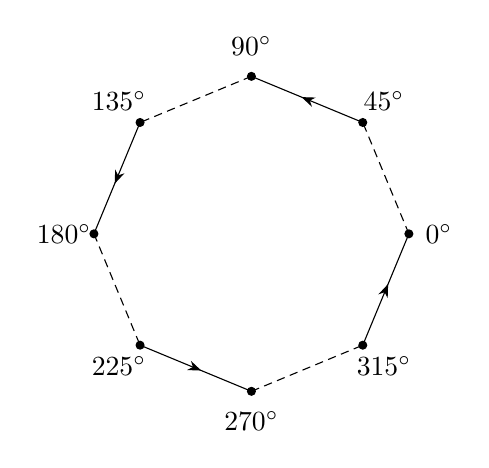
\begin{tikzpicture}[%
        ->-/.style = {%
            decoration = {%
                markings,
                mark = at position 0.55 with \arrow{Stealth}
            },
            postaction = {decorate}
        }
    ]

        % Coordinates for the points (they lie on an octagon).
        \foreach\x in {0, 45, ..., 315}{%

            % The point on the circle, given in polar form using degrees.
            \coordinate (\x) at (\x:2);

            % Add a dot at each point.
            \draw[fill = black] (\x) circle (0.05);

            % Label the point by its angle on the unit circle.
            \node at (\x:2.38) {$\x^{\circ}$};
        }

        % Dashed lines for one action.
        \draw[densely dashed] (0) to (45);
        \draw[densely dashed] (90) to (135);
        \draw[densely dashed] (180) to (225);
        \draw[densely dashed] (270) to (315);

        % Solid lines for the other.
        \draw[->-] (45) to (90);
        \draw[->-] (135) to (180);
        \draw[->-] (225) to (270);
        \draw[->-] (315) to (0);
    \end{tikzpicture}
\end{document}
